\begin{figure}[t]
    \centering
    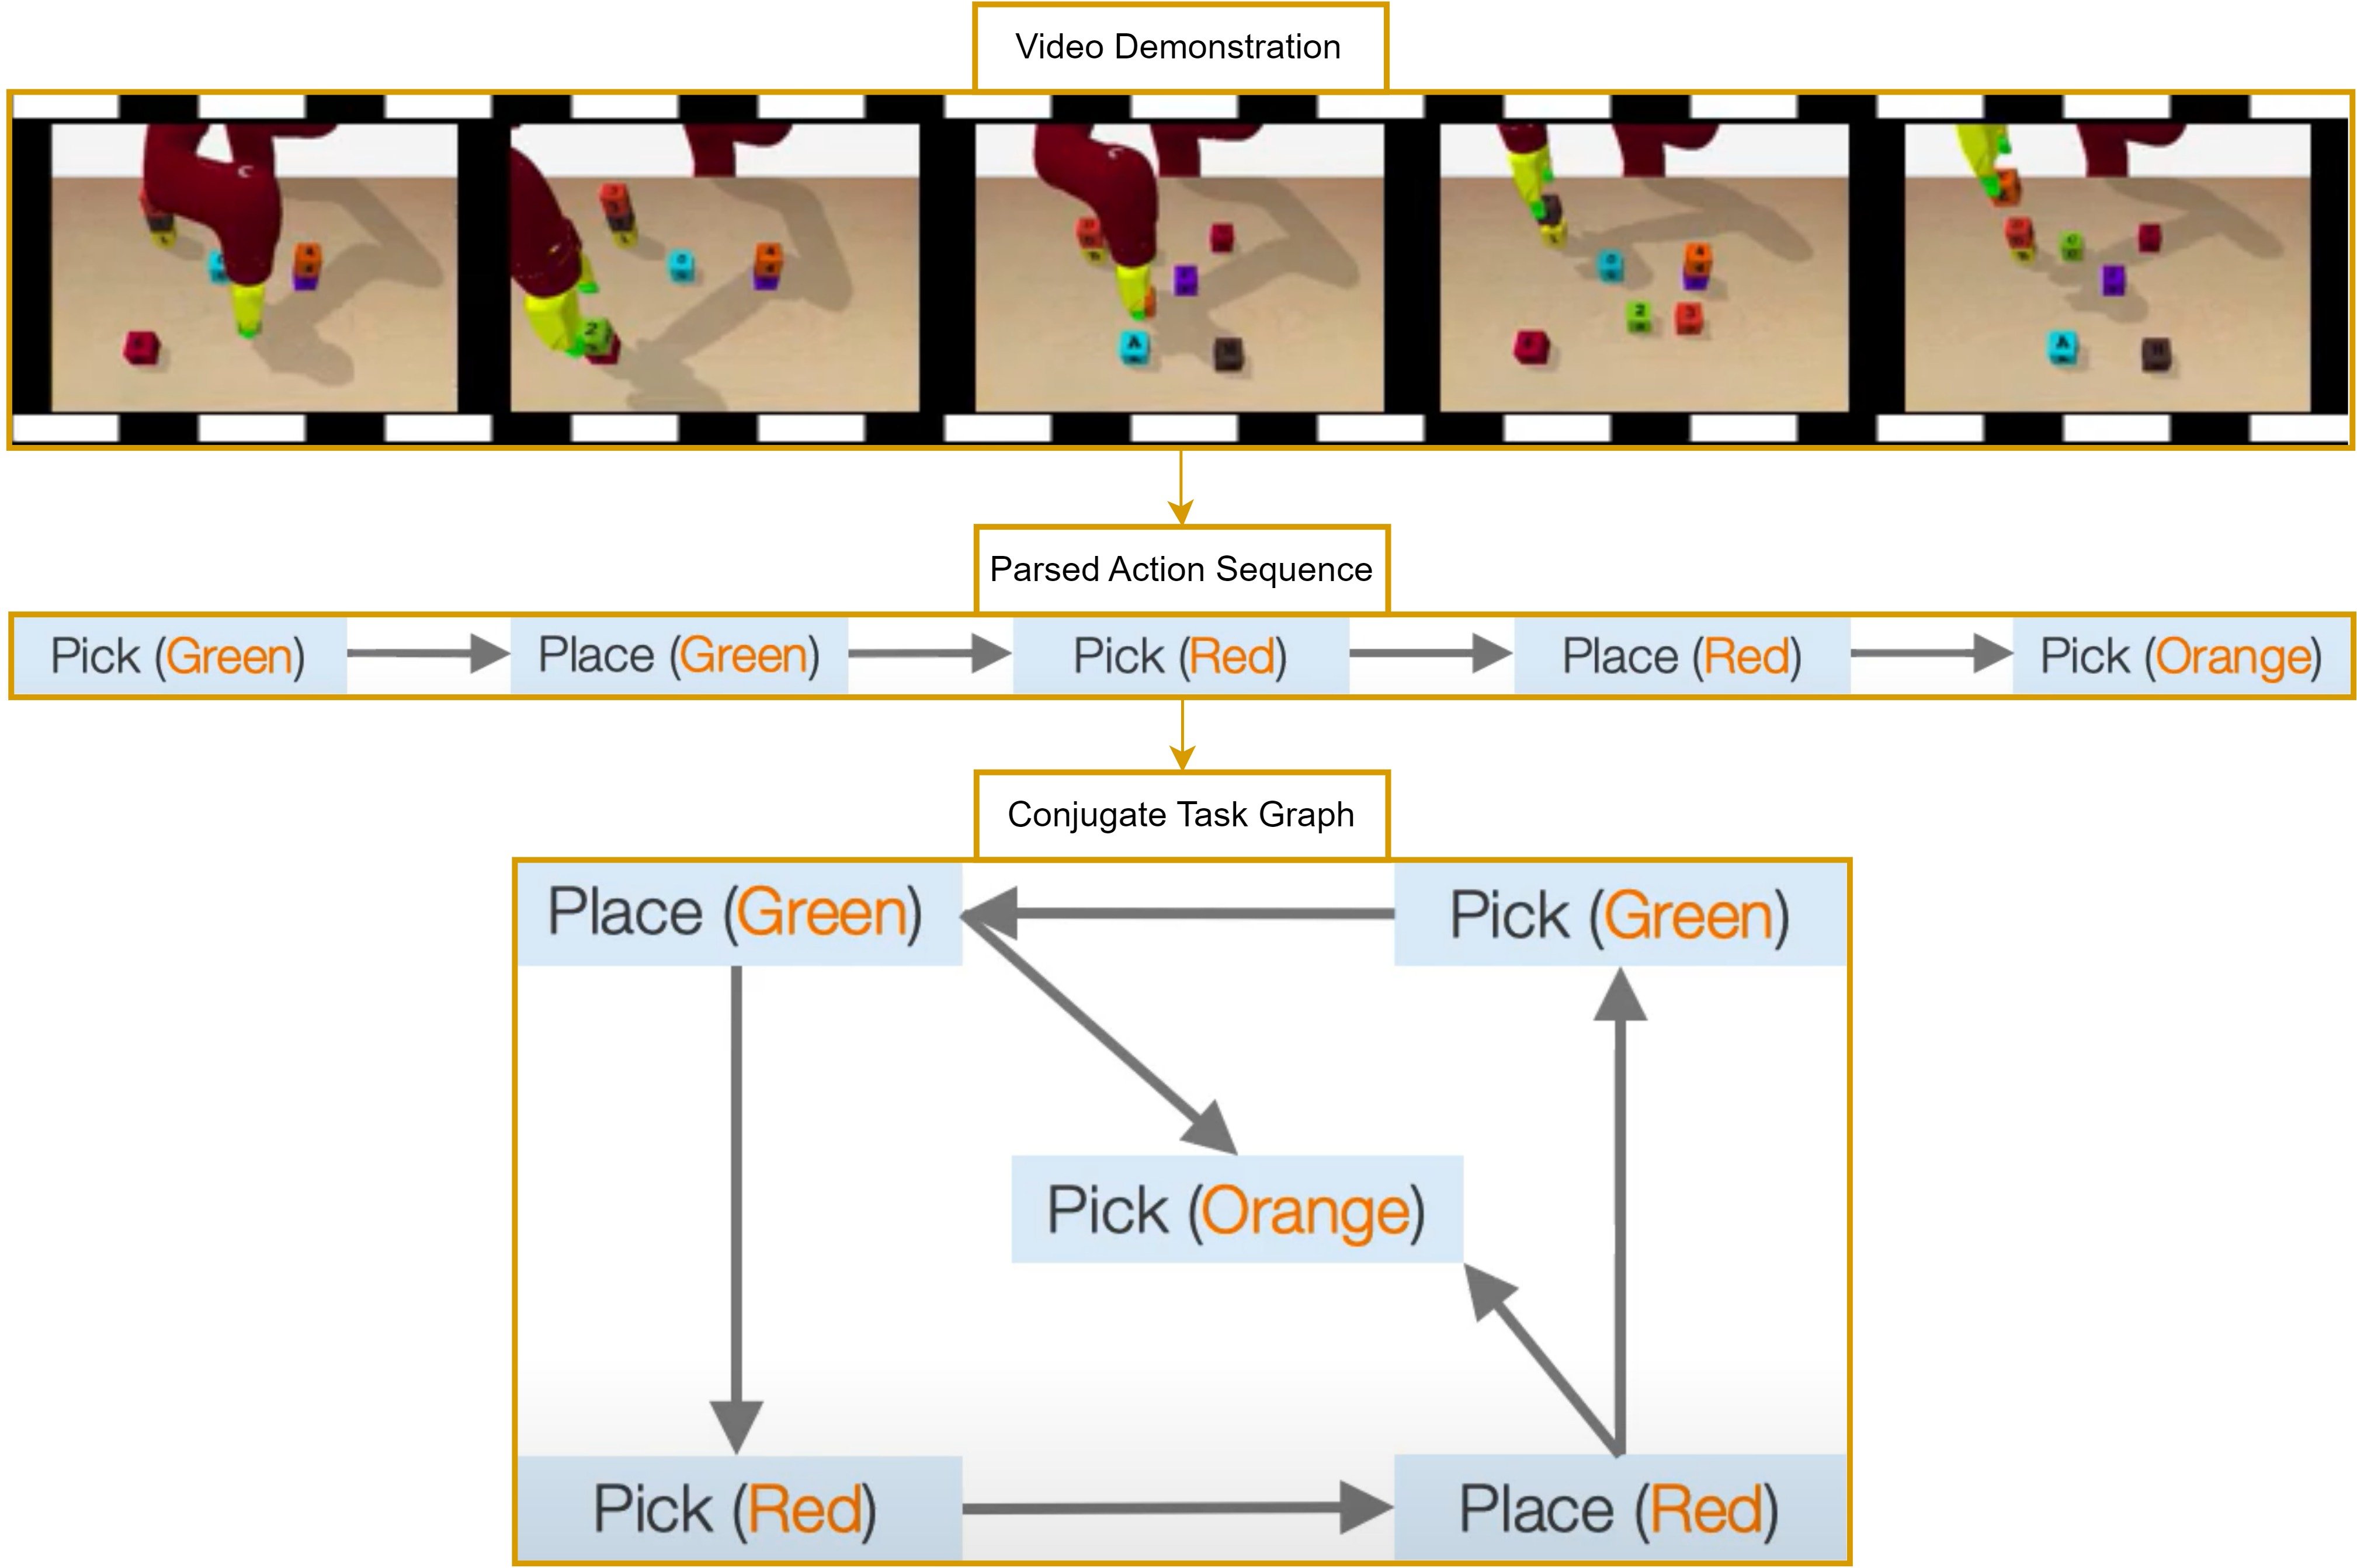
\includegraphics[width=0.8\textwidth]{figures/images/ch4/conjugate_task_graph.jpg}
    \caption{Conjugate Task Graph representation. Starting from the video demonstration, the sequence of actions is extracted and used to construct the initial graph. Then the complete Conjugate Task Graph is built by predicting the missing edges, which represents possible actions sequences observed in the training set.}
    \label{fig:conjugate_task_graph}
\end{figure}
